\documentclass[11pt]{article}
\usepackage[scale=1.5]{ccicons}
\usepackage{url}
\usepackage{array}
\usepackage{multicol}
\usepackage{tabu}
\usepackage[table]{xcolor}
\usepackage{tikz}
\usetikzlibrary{shapes.geometric}
\usepackage{fancyhdr}
\usepackage[margin=.7in]{geometry}
\usepackage[hang,flushmargin,symbol*]{footmisc}
\usepackage{amsmath}
\usepackage{amsthm}
\usepackage{amssymb}
\usepackage{mathtools}
\usepackage{enumitem}
\usepackage{graphicx}
\usepackage{color}
\definecolor{darkblue}{rgb}{0, 0, .6}
\definecolor{grey}{rgb}{.7, .7, .7}
\usepackage[breaklinks]{hyperref}

\theoremstyle{definition} 
\newtheorem{theorem}{Theorem}
\newtheorem{lemma}[theorem]{Lemma}
\newtheorem{claim}[theorem]{Claim}
\newtheorem{corollary}[theorem]{Corollary}
\newtheorem{conjecture}[theorem]{Conjecture}
\newtheorem{definition}[theorem]{Definition}
\newtheorem{example}[theorem]{Example}
\newtheorem{remark}[theorem]{Remark}
\newtheorem{important}[theorem]{Important Note}
\newtheorem{recall}[theorem]{Recall}
\newtheorem{note}[theorem]{Note}
\newtheorem{question}[theorem]{Question}
\newtheorem*{definition*}{Definition}
\newtheorem*{theorem*}{Theorem}
\newtheorem*{claim*}{Claim}

\newcommand{\ds}{\displaystyle}
\newcommand{\Spin}{\operatorname{Spin}}
\newcommand{\Rng}{\operatorname{Rng}}

\DeclareMathOperator{\Aut}{Aut}
\DeclareMathOperator{\Inv}{Inv}
\DeclareMathOperator{\inv}{inv}
\DeclareMathOperator{\Two}{Two}
\DeclareMathOperator{\des}{des}
\DeclareMathOperator{\asc}{asc}
\DeclareMathOperator{\Asc}{Asc}
\DeclareMathOperator{\Des}{Des}
\DeclareMathOperator{\rev}{rev}
\DeclareMathOperator{\runs}{runs}
\DeclareMathOperator{\TL}{TL}
\DeclareMathOperator{\tr}{tr}
\DeclareMathOperator{\Tr}{Tr}
\DeclareMathOperator{\pk}{pk}
\DeclareMathOperator{\coins}{coins}
\DeclareMathOperator{\Dyck}{Dyck}

\newcommand{\euler}[2]{
  \displaystyle \left\langle\begin{matrix}#1  \\#2  \\ \end{matrix}\right\rangle}

\newcommand{\stirling}[2]{
  \displaystyle \left\{\begin{matrix}#1  \\#2  \\ \end{matrix}\right\}}

\setlength{\parindent}{0pt}
\setlength{\fboxsep}{10pt}

%%%%%%Header/Footer%%%%%%%

\pagestyle{fancy}

\lhead{MAT 526 - Spring 2021}
\chead{}
\rhead{Exam 1 (Part 2)}
\lfoot{\scriptsize This work is licensed under the \href{https://creativecommons.org/licenses/by-sa/4.0/}{Creative Commons Attribution-Share Alike 4.0 License}.} 
\cfoot{}
\rfoot{\ccbysa}
\renewcommand{\headrulewidth}{.4pt}
\renewcommand{\footrulewidth}{.4pt}

%%%%%%%%%%%%%%%%%%%

\begin{document}

\tikzstyle{vert} = [circle, draw, fill=grey,inner sep=0pt, minimum size=6mm]
\tikzstyle{vertsmall} = [circle=3pt, draw, fill=grey]
\tikzstyle{s} = [draw, very  thick, black, stealth-stealth]
\tikzstyle{s1} = [draw, very  thick, black,-stealth]
\tikzstyle{d} = [draw, very  thick, black, dashed,-stealth]
\tikzstyle{d2} = [draw, very thick, dashed,stealth-stealth]
\tikzstyle{s2} = [draw, very thick, stealth-stealth]
\tikzstyle{snake} = [draw, very thick, snake it,-stealth]
\tikzstyle{snake2} = [draw, very thick, snake it, stealth-stealth]
\tikzstyle{g} = [draw, very thick, grey,-stealth]
\tikzstyle{g2} = [draw, very thick, grey, stealth-stealth]

\begin{center}

{\Large\bf Exam 1 (Part 2)}

\bigskip

  \fbox{\parbox{7in}{
    \vspace{5pt}
    \textbf{\large Your Name:}
    \vspace{5pt}
  }}
  
  \bigskip
  
  \fbox{\parbox{7in}{
    \vspace{5pt}
    \textbf{\large Names of Any Collaborators:}
    \vspace{5pt}
  }}

\end{center}

\section*{Instructions}

Answer each of the following questions and then submit your solutions to BbLearn by \textbf{11:59\textsc{pm} on Friday, March 5}. You can either write your solutions on paper and then capture your work digitally or you can write your solutions digitally on a tablet (e.g., iPad). This part of Exam 1 is worth a total of 16 points and is worth 40\% of your overall score on Exam 1. Your overall score on Exam 1 is worth 25\% of your overall grade.

\bigskip

I expect your solutions to be \emph{well-written, neat, and organized}.  Do not turn in rough drafts.  What you turn in should be the ``polished'' version of potentially several drafts.  Feel free to type up your final version.  The \LaTeX\ source file of this exam is also available if you are interested in typing up your solutions using \LaTeX.  I'll gladly help you do this if you'd like.

\bigskip

Reviewing material from previous courses and looking up definitions and theorems you may have forgotten is fair game. However, when it comes to completing the following problems, you should \emph{not} look to resources outside the context of this course for help.  That is, you should not be consulting the web, other texts, other faculty, or students outside of our course in an attempt to find solutions to the problems you are assigned.  This includes Chegg and Course Hero. On the other hand, you may use each other, the textbook, me, and your own intuition. Further information:
\begin{enumerate}
\item You may freely use any theorems that we have discussed in class, but you should make it clear where you are using a previous result and which result you are using.  %For example, if a sentence in your proof follows from Problem 3.16, then you should say so.
\item Unless you prove them, you cannot use any results from the course notes/book that we have not yet covered.
\item You are \textbf{NOT} allowed to consult external sources when working on the exam.  This includes people outside of the class, other textbooks, and online resources.
\item You are \textbf{NOT} allowed to copy someone else's work.
\item You are \textbf{NOT} allowed to let someone else copy your work.
\item You are allowed to discuss the problems with each other and critique each other's work.
\end{enumerate}

\begin{center}
\textbf{I will vigorously pursue anyone suspected of breaking these rules.}
\end{center}

You should \textbf{turn in this cover page} and all of the work that you have decided to submit. \textbf{Please write your solutions and proofs on your own paper.} To convince me that you have read and understand the instructions, sign in the box below.

\bigskip

  \fbox{\parbox{7in}{
    \vspace{5pt}
    \textbf{\large Signature:} \hfill
    \vspace{5pt}
  }}

\bigskip

Good luck and have fun!

\newpage

\begin{enumerate}
	
\item (4 points each) Complete \textbf{one} of the following.
\begin{enumerate}
\item Prove that $C_n$ counts the number of ways we can stack coins in the plane such that the bottom row consists of $n$ consecutive coins.  You should think of this as the two-dimensional version of stacking apples.  For example, here are all the ways to stack coins so that the bottom row has 3 coins.
\begin{center}
\includegraphics[width=3.5in]{coins.png}
\end{center}

\item Consider a rectangle with $n$ nodes across the top edge and $n$ nodes across the bottom edge.  A \emph{Temperley--Lieb $n$-diagram} in the rectangle consists of $n$ edges connecting the $2n$ nodes such that:
\begin{itemize}
\item each edge connects a pair of nodes,
\item each node is connected to exactly one edge,
\item the edges must be drawn inside the rectangle,
\item none of the edges are allowed to cross or touch.
\end{itemize}
Below is an example of a 6-diagram.

\begin{center}
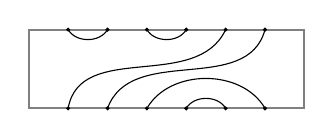
\begin{tikzpicture}[scale=.5]
\draw[gray,thick] (0,0) rectangle (7,2);
\foreach \x in {1,2,3,4,5,6} \filldraw (\x,0) circle (1pt);
\foreach \x in {1,2,3,4,5,6} \filldraw (\x,2) circle (1pt);
\draw (3,0) to [bend left=60] (6,0);
\draw (2,0) to [out=70,in=-105] (6,2);
\draw (4,0) to [bend left=60] (5,0);
\draw (1,2) to [bend right=60] (2,2);
\draw (1,0) to [out=80,in=-115] (5,2);
\draw (3,2) to [bend right=60] (4,2);
\end{tikzpicture}
\end{center}
Let $\TL(n)$ denote the collection of $n$-diagrams. Prove that $|TL(n)|=C_n$.

\item Tickets to a show are 50 cents and $2n$ customers stand in a queue at the ticket window.  Half of them have \$1 and the others have 50 cents.  The cashier starts with no money. How many arrangements of the queue are possible with the proviso that the cashier always be able to make change?

\end{enumerate}

\item (4 points each) Complete \textbf{two} of the following.
\begin{enumerate}

\item Let $L(k,n-k)$ denote the set of lattice paths $p$ from $(0,0)$ to $(k,n-k)$ consisting of only North steps and East steps. Note that each path in $L(k,n-k)$ consists of $k$ East steps and $n-k$ North steps for a total of $n$ steps. Prove that there is a bijection between $L(k,n-k)$ and the set $\{w\in S_n\mid \Des(w)\subseteq \{k\}\}$.

\item For $w=w(1)\cdots w(n)\in S_n$ define the \emph{trace} of $w$, denoted $\tr(w)$, to be the sum of the positions of the descents of $w$. Prove that
\[
\sum_{w\in S_n}t^{\tr(w)}=\sum_{w\in S_n}t^{\inv(w)}.
\]
\emph{Note:} If $\Tr_n(t)$ is the generating function for the number of permutations in $S_n$ with trace equal to $k$, we have shown that $\displaystyle \Tr_n(t)=\frac{\prod_{i=1}^n(1-t^i)}{(1-t)^n}$ since this is the formula we found for $I_n(t)$ in Problem~1(g) on Homework~7.

\item The \emph{wicked awesome sorting length} of a permutation $w=w(1)\cdots w(n)\in S_n$, denoted $\ell(w)$, to be the minimal number of adjacent swaps of positions needed to sort the permutation to the identity. For example, $31542$ has wicked awesome sorting length at most 5 since the permutation can be unscrambled in five moves as follows:
\[
31\underline{54}2 \to 314\underline{52} \to 31\underline{42}5 \to \underline{31}245 \to 1\underline{32}45 \to 12345.
\]
In fact, $\ell(31542)$ is exactly 5. Prove that $\inv(w)=\ell(w)$ for all $w\in S_n$. \emph{Hint:} Start by proving that applying an adjacent swap to positions of a permutation either increases the number of inversions by one or decreases the number of inversions by one, and then describe an unscrambling algorithm that decreases the number of inversions after each swap.

\item (Hanoi Solitaire) Consider a deck of $n$ cards labeled $1,2,\ldots, n$. An arrangement of the cards is denoted $c_1c_2\cdots c_n$, where $c_1$ is the number corresponding to the top card and $c_n$ is the number corresponding to the bottom card.  We now describe a type of solitaire involving three piles of cards. Our starting configuration is an empty left pile, $c_1c_2\cdots c_n$ in the middle, and an empty right pile. We then employ the following algorithm:
\begin{enumerate}
\item[(1)] Move the current top card $c_i$ of the middle pile to the top of the left pile if the left pile is empty or if $c_i$ is smaller than the current top card $c_j$ of the left pile.
\item[(2)] Otherwise, move the top card $c_j$ from the left pile to the bottom of the right pile. 
\end{enumerate}
Let $h(c_1c_2\cdots c_n)$ denote the final arrangement of the cards in the right pile. We say that $c_1c_2\cdots c_n$ is a \emph{winning arrangement} if $h(c_1c_2\cdots c_n)=12\cdots n$, and otherwise, $c_1c_2\cdots c_n$ is called a \emph{losing arrangement}. If $n$ is the $i$th card, first prove that 
\[
h(c_1\cdots c_{i-1}nc_{i+1}\cdots c_n)=h(c_1\cdots c_{i-1})h(c_{i+1}\cdots c_n)n,
\]
and then use this to find the number of winning arrangements of $n$ cards. \emph{Hint:} Induction could come in handy depending on your approach. \emph{Note:} This problem is awesome!

\end{enumerate}

\item (4 points) Complete \textbf{one} of the following.
\begin{enumerate}
\item A \emph{set composition} of a set $S$ is a set partition with an ordering on its blocks. When writing a set composition of $[n]$, it is standard practice to write the elements in each block in increasing order. This allows us to abbreviate a set composition of $[n]$ as a sequence of increasing runs separated by vertical bars. For example, the set composition $(\{3\},\{4,6\},\{1,5,2\})$ would be written as $3|46|125$. Using this model, each set composition of $[n]$ is associated with a permutation on $n$. For example, the ``underlying" permutation in the example above is $346125$. Notice that each permutation $w\in S_n$ is associated with potentially many set compositions and we must always place a bar in a descent position. Moreover, we can place additional bars in the gaps between numbers in the permutation, but we are only allowed to place a single bar (since blocks must be nonempty). Let $\mathcal{C}(w)$ denote the collection of set compositions with underlying permutation $w$. Prove that
\[
\sum_{C\in\mathcal{C}(w)}t^{|C|}=t^{\runs(w)}(1+t)^{n-\runs(w)},
\]
where $|C|$ denotes the number of blocks in the set composition $C$ and $\runs(w)$ is the number of maximal increasing runs in $w$.

\item Recall definition of derangements and the corresponding sequence $d_n$ given on Part 1 of Exam 1. Find a closed form for the exponential generating function for $d_n$:
\[
D(z):=\sum_{n\geq 0}d_n\frac{z^n}{n!}.
\]

\item Let $\coins_n$ be the number of ways to make change for $n$ cents using pennies, nickels, dimes, and quarters. Let $F_{\coins}(z)$ be the generating function for $\coins_n$:
\[
F_{\coins}(z):=\sum_{n\geq 0}\coins_nz^n.
\]
Prove that 
\[
F_{\coins}(z)=\frac{1}{(1-z)(1-z^5)(1-z^{10})(1-z^{25})}.
\]

\end{enumerate}

\end{enumerate}

\textbf{Bonus Question!} (2 points) This question is optional.  Use a computer algebra system (e.g., WolframAlpha, Mathematica, Sage/CoCalc, Maple, etc.) together with the expression for $F_{\coins}(z)$ to find the number of ways to make change for \$1.

%scraps: 

%\item Prove that a permutation $w\in S_n$ is uniquely determined by its inversion set $\Inv(w)$.

%\item Stirling numbers of the first kind (see IBL pages 59--63).

%\item Prove that the number of sequences consisting of $n$ ones and $n$ negative ones such that every partial sum is nonnegative is $C_n$.

%\item The book describes a bijection from $S_n(231)$ to $\Dyck(n)$ in Section~2.4.3, which shows that $C_n=|S_n(231)|=|\Dyck(n)|$. However, many details are missing.  A \emph{peak} of a Dyck path $p$ is a point $(i,j)$ along the path in the plane such that $(i,j-1)$ and $(i+1,j)$ are also on $p$. In other works, a peak occurs at a point along the path where there is a North step following by an East step. Let $\pk(p)$ denote the number of peaks on the Dyck path $p$.
%\begin{enumerate}
%\item Explain why reversing the map $\psi$ defined in the book will yield a 231-avoiding permutation.
%\item Prove that $\displaystyle C_n(t)=\sum_{p\in \Dyck(n)}t^{\pk(p)-1}$.
%\end{enumerate}

%\item Explain why $0\leq \tr(w)\leq \binom{n}{2}$ for all $w\in S_n$.


\end{document}